% \chapter{Sistema Proposto}
% \chapter{Sistema de recuperação de informação em documentos multi-tópicos}
\chapter{Sistema de Recuperação de Informação em Documentos Multi-temáticos}
\label{cap3}


O sistema proposto tem como objetivo recuperar informações em uma coleção de documentos em que cada documento contém assuntos diversos e relativamente independentes entre si. Esse sistema deve identificar os assuntos de cada documento e disponibilizá-los de forma que o usuário consiga consultar a coleção de documentos e obter todo o histórico de ocorrências de um determinado tema de forma que possa identificar onde esse tema foi mencionado, bem como se houve uma decisão relacionada ao tema. Os documentos constituídos por diversos assuntos, são aqui chamados de documentos multi-temáticos, em contraste com aqueles cujo assunto central é bem definido e constante ao logo do texto.  

A proposta original deste trabalho contempla funcionalidades de classificação para identificar automaticamente o tipo de ocorrência onde um assunto é mencionado, o qual pode ser classificado como uma decisão, informe ou simplesmente uma menção ao assunto. Contudo essas funcionalidades configuram trabalhos futuros para continuação do sistema como concebido inicialmente. Assim, esse trabalho de mestrado está focado na segmentação de atas de reunião, no agrupamento desses segmentos em tópicos e na recuperação de trechos de atas relacionados ao assunto da pesquisa.

Esse capítulo está organizado da seguinte forma: primeiramente, na Seção~\ref{sec:sistema-proposto} é apresentada uma visão geral do sistema proposto, seu funcionamento e como as técnicas de segmentação textual e extração de tópicos são empregadas para gerar uma base de dados que concentra as informações necessárias para identificar e agrupar os diversos assuntos distribuídos na coleção de documentos. Ainda nessa seção, é apresentada a utilização das técnicas de recuperação de informação empregadas para entregar os segmentos de acordo com a consulta do usuário bem como permitir a exploração de segmentos relacionados ao mesmo tema, os quais originalmente estão distribuídos na coleção de documentos.  
Na Seção~\ref{sec:aplicacao-sistema} é apresentada a aplicação do sistema proposto utilizando como base de dados uma coleção de atas de reunião. Uma vez que as atas configuram um \textit{corpus} com documentos multi-temáticos, o sistema as utilizará e as técnicas empregadas serão analisadas. Ainda nessa seção, será apresentada a preparação das atas, bem como a descrição dos algoritmos utilizados e suas configurações.






\section{Sistema Proposto}
\label{sec:sistema-proposto}

Essa Seção apresenta as etapas de desenvolvimento do sistema de recuperação de atas proposto, bem como o seu funcionamento geral, desde a preparação dos documentos até a entrega dos resultados ao usuário. 
Na Figura \ref{fig:visao-geral} é mostrada a visão geral do sistema com suas principais entradas e saídas. Inicialmente o sistema recebe um conjunto inicial de documentos por meio do Módulo de preparação/manutenção cuja função é processar e manter esses textos para gerar uma base de dados interna que codifica os textos extraídos com seus respectivos tópicos. Essa base de dados fica disponível ao Módulo de Consulta recebe a entrada pela qual o usuário expressa um assunto de interesse. Em seguida, os trechos de texto que fazem menção ao esse assunto são exibidos ao usuário.


  %--- Figura Visão Geral ---
  \begin{figure}[!h]
	  \centering
	  % \includegraphics[width=0.85\textwidth]{conteudo/capitulos/figs/visão-geral-4.pdf}
	  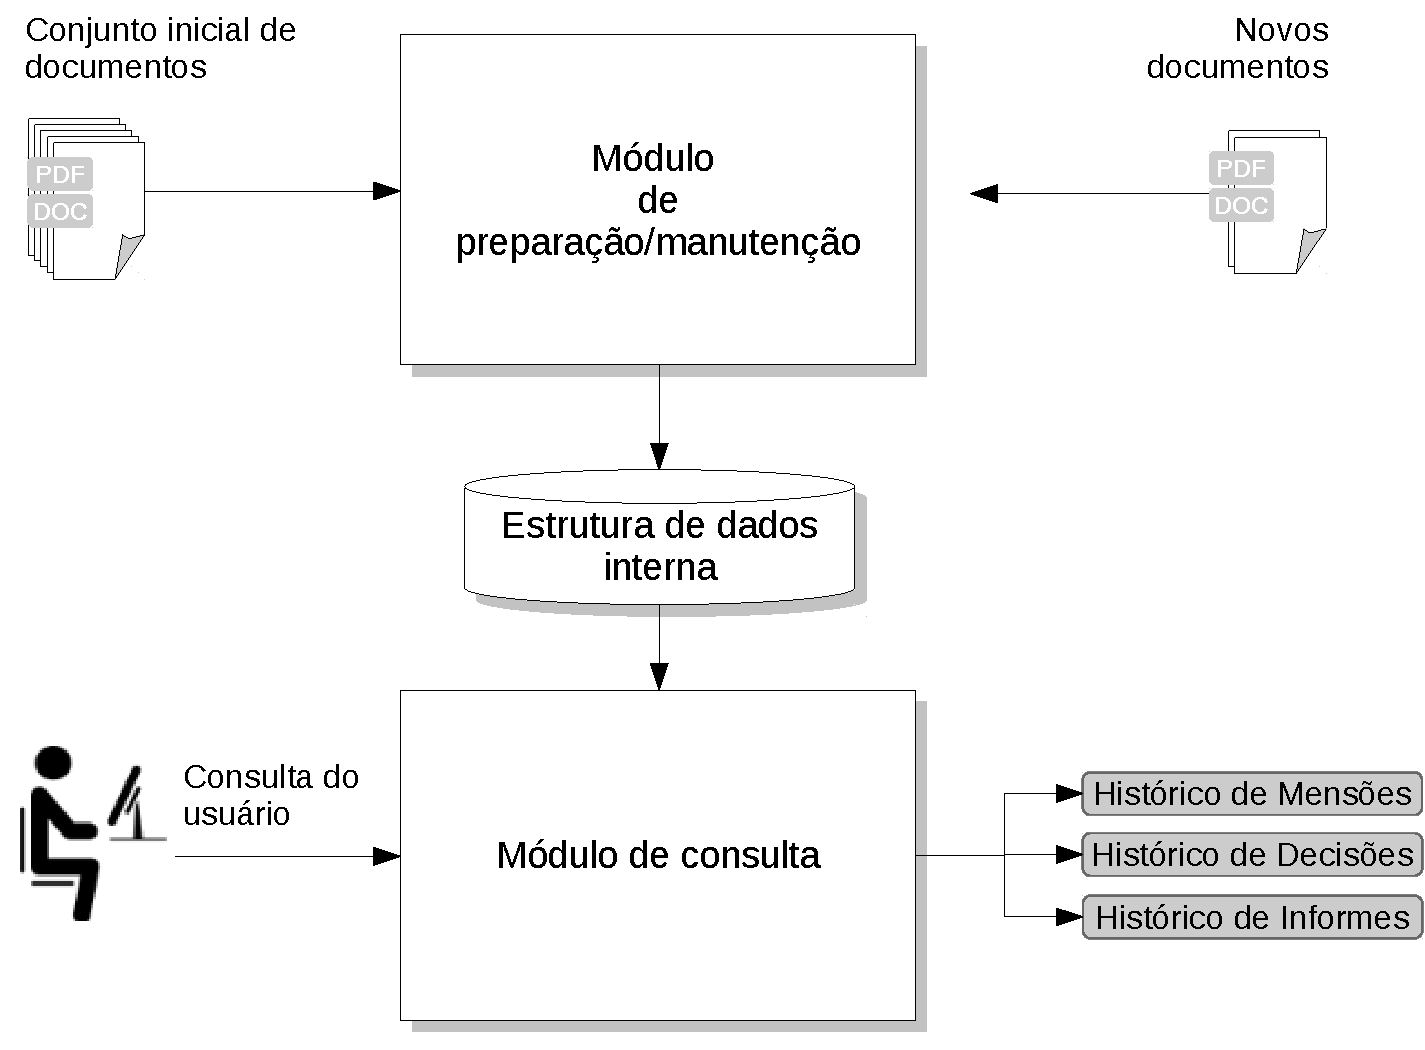
\includegraphics[trim={ 0 0 0 0 },clip,page=1,width=.8\textwidth]{conteudo/capitulos/figs/visao-geral-4.pdf}
	  \caption{Visão geral do sistema.}
	  \label{fig:visao-geral}
  \end{figure}

% visão-geral-4






% ========== Módulo de Preparação e manutenção ==========

\subsection{Módulo de Preparação e Manutenção}\label{sec:modulo-preparacao}

O módulo de preparação e manutenção tem como função principal manter uma base de dados necessária para os processos de Recuperação de Informação e Aprendizado de Máquina. Primeiramente, esse módulo deve receber um conjunto inicial de documentos e em seguida organizá-lo por meio das técnicas de segmentação textual e extração de tópicos, de forma que o conjunto resultante formado por segmentos de documentos e os dados obtidos pelo extrator de tópicos constitua um novo \textit{corpus} estruturado e mais adequado às técnicas de Recuperação de Informação e Aprendizado de Máquina. Além disso, considera-se o crescimento da bases de documentos, assim, o sistema deve receber novos documentos a medida que são gerados. A seguir são detalhadas as etapas do Módulo de preparação e manutenção desde a preparação dos documento até a entrega da base de dados interna ao Módulo de Consulta. 

% melhorar ↓↓↓↓↓

% Inicialmente serão descritos a seleção e pré-processamento das atas. 



% ========== Preparação dos Documentos ==========

\subsubsection{Preparação dos Documentos}


Os documentos são normalmente armazenadas em arquivos binários do tipo \textit{pdf}, \textit{doc}, \textit{docx} ou \textit{odt}. A partir desses arquivos, os textos devem ser pré-processados e estruturadas para que possam ser aplicados métodos de Mineração de Texto e Recuperação de Informação. Para isso, o texto plano é extraído e passa por processos de transformação que incluem remoção de elementos considerados menos significativos e a identificação de sentenças. Esse processo é ilustrado na Figura~\ref{fig:preprocessamento-segmentacao} e descrito a seguir.

\begin{center}
	\begin{figure}[h!]

		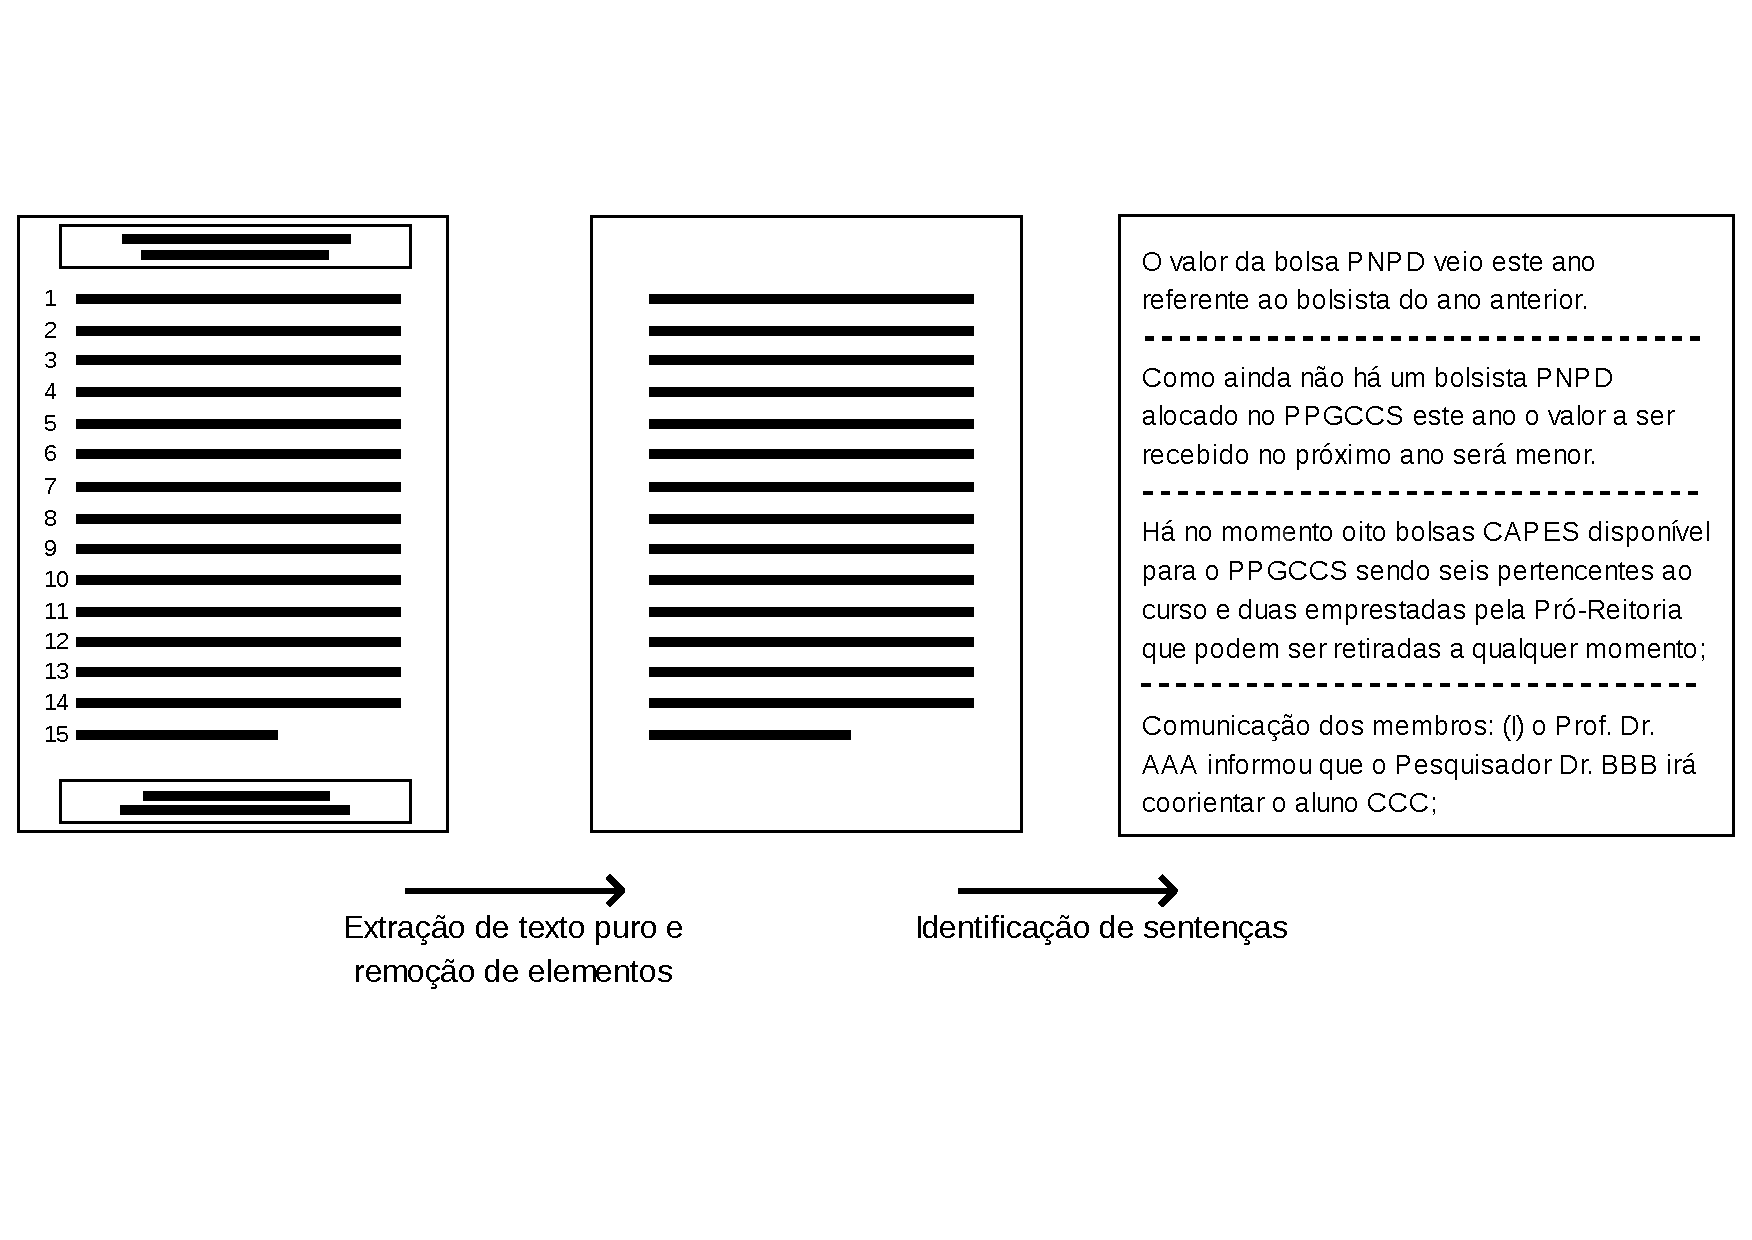
\includegraphics[trim={ 0 100 0 100 },clip,page=1,width=\textwidth]{conteudo/capitulos/figs/preparacao-docs.pdf}

		\caption{Etapa de preparação de um documento que inclui da extração de texto puro,  remoção de elementos menos significativos e a identificação de sentenças.}
		\label{fig:preprocessamento-segmentacao}
	\end{figure}
\end{center}


% -> Essa imagem deve ser mais completa. desde a extração dos textos até os subdocumentos;


%  Cabeçalhos e rodapés
% Remoção de cabeçalhos: 
É frequente que alguns documentos, como as atas de reunião, contenham trechos que podem ser considerados pouco informativos e descartados durante o pré-processamento, como cabeçalhos e rodapés que se misturam aos tópicos tratados na reunião, podendo ser inseridos no meio de um tópico prejudicando tanto os algoritmos de Mineração de Texto e Recuperação de Informação, quanto a leitura do texto pelo usuário. Um cabeçalho é a porção de texto que inicia cada página do documento e, de forma semelhante, um rodapé e a porção que as encerra. Detecta-se os cabeçalhos e os rodapés sempre que há uma repetição das primeiras e últimas palavras do documento, comummente no início e final de cada página. Uma vez identificadas, essas repetições são consideradas irrelevantes e removidas.


%  Identificação de sentenças
% \item 
% Identificação sentenças: 
Nesse trabalho considera-se as sentenças as menores unidades de informação a serem processadas pelos algoritmos de segmentação, por tanto, estas devem ser identificadas. Ao considerar intuitivamente que uma sentença seja uma sequência de palavras entre sinais de pontuação como ``.'', ``!'' e ``?'', alguns erros poderiam ocorrer quando esses tiverem outra função dentro do texto como em abreviações\footnote{As abreviações são identificadas por meio de uma lista com 234 abreviações conhecidas.}, endereços de internet e datas. Outro problema seriam frases curtas com poucas palavras e que não expressam um conceito completo, mas parte dele. Devido ao estilo de pontuação desses documentos, como encerrar sentenças usando um ``;'' e inserção de linhas extras, foram usadas as regras especiais para identificação de finais de sentença. No Algoritmo~\ref{alg:identificacaofinaisdesent} é mostrado como cada \textit{token}\footnote{Nesse trabalho um \textit{token} é qualquer conjunto de símbolos entre sinais não visuais como espaços, quebras de linha e tabulações.} é identificado  como final de sentença.  % Os detalhes sobre essas regras estão disponíveis para consulta em \urlsoftwares.



\begin{algorithm}
	\SetKwInOut{Input}{Entrada}
	\SetKwInOut{Output}{Saída}
	\SetKwBlock{Inicio}{início}{fim}
	\SetKwFor{ParaTodo}{para todo}{}{fim para todo}
	\SetKwIF{Se}{SenaoSe}{Senao}{}{}{senao se}{senao}{fim se}
	\SetKwFor{Para}{}{}{}
%	\SetKwAlgorithm{Algorithm}{Algoritmo}{}

	
	\Input{Texto}
	\Output{Texto com identificações de finais de sentença}
	
	\ParaTodo {token, marcá-lo como final de sentença se:} {	

	Terminar com um \texttt{!}\\
	Terminar com um \texttt{.} e não for uma abreviação\\
	Terminar em \{`\texttt{.}', `\texttt{?}', `\texttt{;}'\} e:
		\Para{}{
			For seguido de uma quebra de parágrafo ou tabulação\\
			O próximo \textit{token} iniciar com  \{ `(',   `\texttt{\{}',  `\texttt{[}',   `\texttt{"}',    `\texttt{'}'     
			\}  \\
			O próximo \textit{token} iniciar com letra maiúscula\\
			O penúltimo character  for \{ 
			`\texttt{)}',   `\texttt{\}}',   `\texttt{]}',   `\texttt{"}',   `\texttt{'}'
			\}\\
		}
	}
	
	\caption{Identificação de finais de sentença.}
	\label{alg:identificacaofinaisdesent}
\end{algorithm}

% \end{enumerate}
	



% ========== Pré-Processamento dos Documentos ==========


\subsubsection{Pré-Processamento dos Documentos}



Nessa etapa os documentos são pré-processados individualmente antes de serem recebidos pelos algoritmos de segmentação e extração de tópicos. Inicialmente, cada texto passa por um processo de transformação em que as letras são convertidas em caixa baixa e elimina-se sinais de pontuação, numerais e termos menores que três caracteres. Em seguida remove-se os termos que não contribuem para a etapa de segmentação, as quais são chamadas de \textit{stop words}. Para identificá-las usa-se uma lista de 438 palavras conhecidas do idioma português, como preposições, artigos e verbos de estado e adicionalmente uma lista contendo palavras muito frequentes e pouco significantes desse domínio com como \textit{``universidade''}, \textit{``computação''} e nomes de pessoas as quais formam listadas manualmente. Em seguida, extrai-se o radical de cada palavra por meio da técnica \textit{stemming} implementada no algoritmo de Porter~\cite{Porter1997}. A etapa de pré-processamento cria uma base de dados intermediária, da qual foram removidos os elementos mencionados. Essa estrutura é utilizada para representar os textos, contudo, a base de dados interna preserva os elementos removidos para apresentação adequada ao usuário.
 
% Nesse trabalho, todos os termos restantes após a remoção de \textit{stop words} e \textit{stemming} foram mantidas independentemente de valores de   \textit{Document Frequency} devido a característica das atas de possuir múltiplos assuntos em um documento. Cada segmento pode ser considerado como um sub-documento quem contém um assunto relativamente independente. 







% Uma imagem para o pré-processamento


% Uma tabela com as modificações

		% Documento | Total de Termos | Termos removidos | Termos com DF >= 2





% ==================== Segmentação ===================== %
\subsubsection{Segmentação}

Como já mencionado, uma ata registra a sucessão de assuntos discutidos em uma reunião, porém apresenta-se com poucas quebras de parágrafo e sem marcações de estrutura, como capítulos, seções ou quaisquer indicações sobre o assunto do texto. Portanto, faz-se necessário descobrir quando há uma mudança de assunto no texto da ata. Para essa tarefa, as técnicas de segmentação de texto recebem uma lista de sentenças, a qual considera cada ponto entre duas sentenças como candidato a limite entre segmentos, ou seja, um ponto onde há transição entre assuntos~\cite{Bokaei2016}. Como resultado, para cada documento tem-se um conjunto de segmentos com um assunto relativamente independente que constituem o texto do documento original, contudo, sem indicações do teor dos segmentos. Em seguida, esses segmentos são processados por um extrator de tópicos que irá agrupá-los por assuntos e eleger palavras para descrever esses tópicos.

% Uma vez identificadas as transições de assuntos 
% As técnicas de segmentação abordadas na Subseção~\ref{sec:segmentacao} dividem o texto de cada ata em segmentos que contêm um assunto relativamente independente. Esses segmentos serão 




% ==================== Extração de Tópicos ===================== %

\subsubsection{Extração de Tópicos}

Após a segmentação da coleção e identificação das transições de assuntos em cada documento da coleção, o sistema inicia a etapa de extração de padrões por meio das técnicas de extração de tópicos, ou seja, uma vez identificado onde há uma mudança de assunto, o próximo passo é obter o tópico ao qual o assunto pertence.

O resultado do processo de extração de tópicos é a representação dos documentos e seus tópicos em uma matriz documento-tópico que atribui um peso a cada tópico para cada documento e uma matriz termo-tópico que pode representar a probabilidade de ocorrência do termo quando um tópico ocorre em um documento ou a frequência esperada desse termo.  
Nesse sistema, essas representações são utilizadas para melhorar as tarefas de recuperação de informação e agrupamento dos documentos. 
O agrupamento por tópicos e seus descritores são utilizados para ajudar o usuário a analisar e identificar os segmentos conforme sua consulta, bem como encontrar resultados similares. 
Após a etapa de extração de tópicos aplicada a um conjunto de segmentos,  cria-se uma base de dados derivada do \textit{corpus} original, a qual é descrita na seção a seguir.



% O processo de extração de tópicos 


% --> explicar o que são descritores;
% os descritores são utilizados;


% ==================== Estrutura de Dados Interna ===================== %

\subsection{Base de Dados Interna}

A base de dados interna é o resultado dos processos de segmentação e extração de tópicos. Constituída por: 
(1) documentos originais para referência, 
(2) segmentos de texto contendo um assunto relativamente independente,
(3) matrizes documento-tópico e termo-tópico.
Na Figura~\ref{fig:estrutura-dados-interna} é apresentado a visão geral da base de dados interna onde ilustra-se os arquivos da coleção de documentos ($D$) que contêm assuntos diversos (representados pelos círculos, quadrados e triângulos) ficando disponíveis para visualização e fonte original das informações. 
% Os arquivos originais são mantidos para referência aos textos integrais ficando disponíveis para visualização e fonte original das informações. 


% deve ser atualizada a cada novo documento inserido no sistema.



	\begin{figure}[h!]
\center
		% 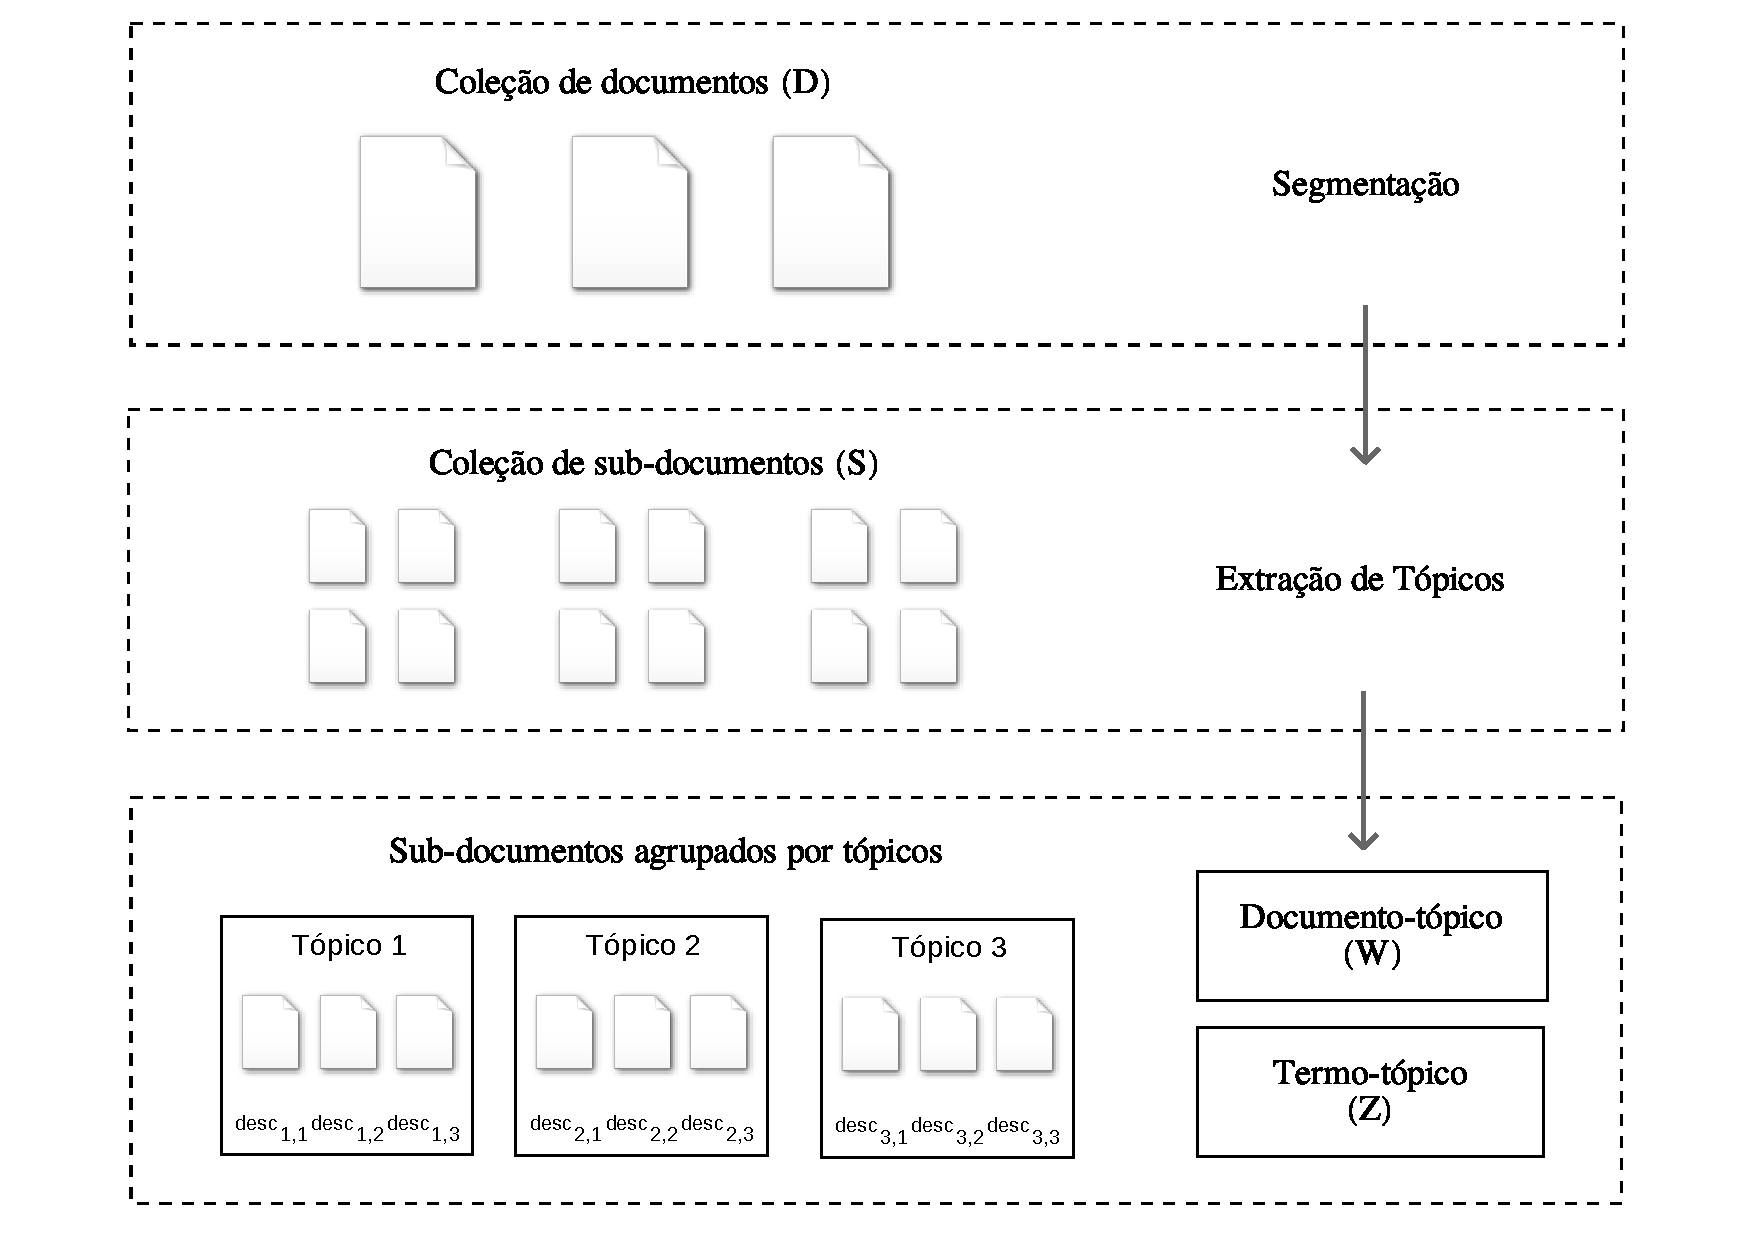
\includegraphics[trim={ 61 0 61 0 },clip,page=1,width=0.9\textwidth]{conteudo/capitulos/figs/estrutura-de-dados-interna.pdf} 
		% 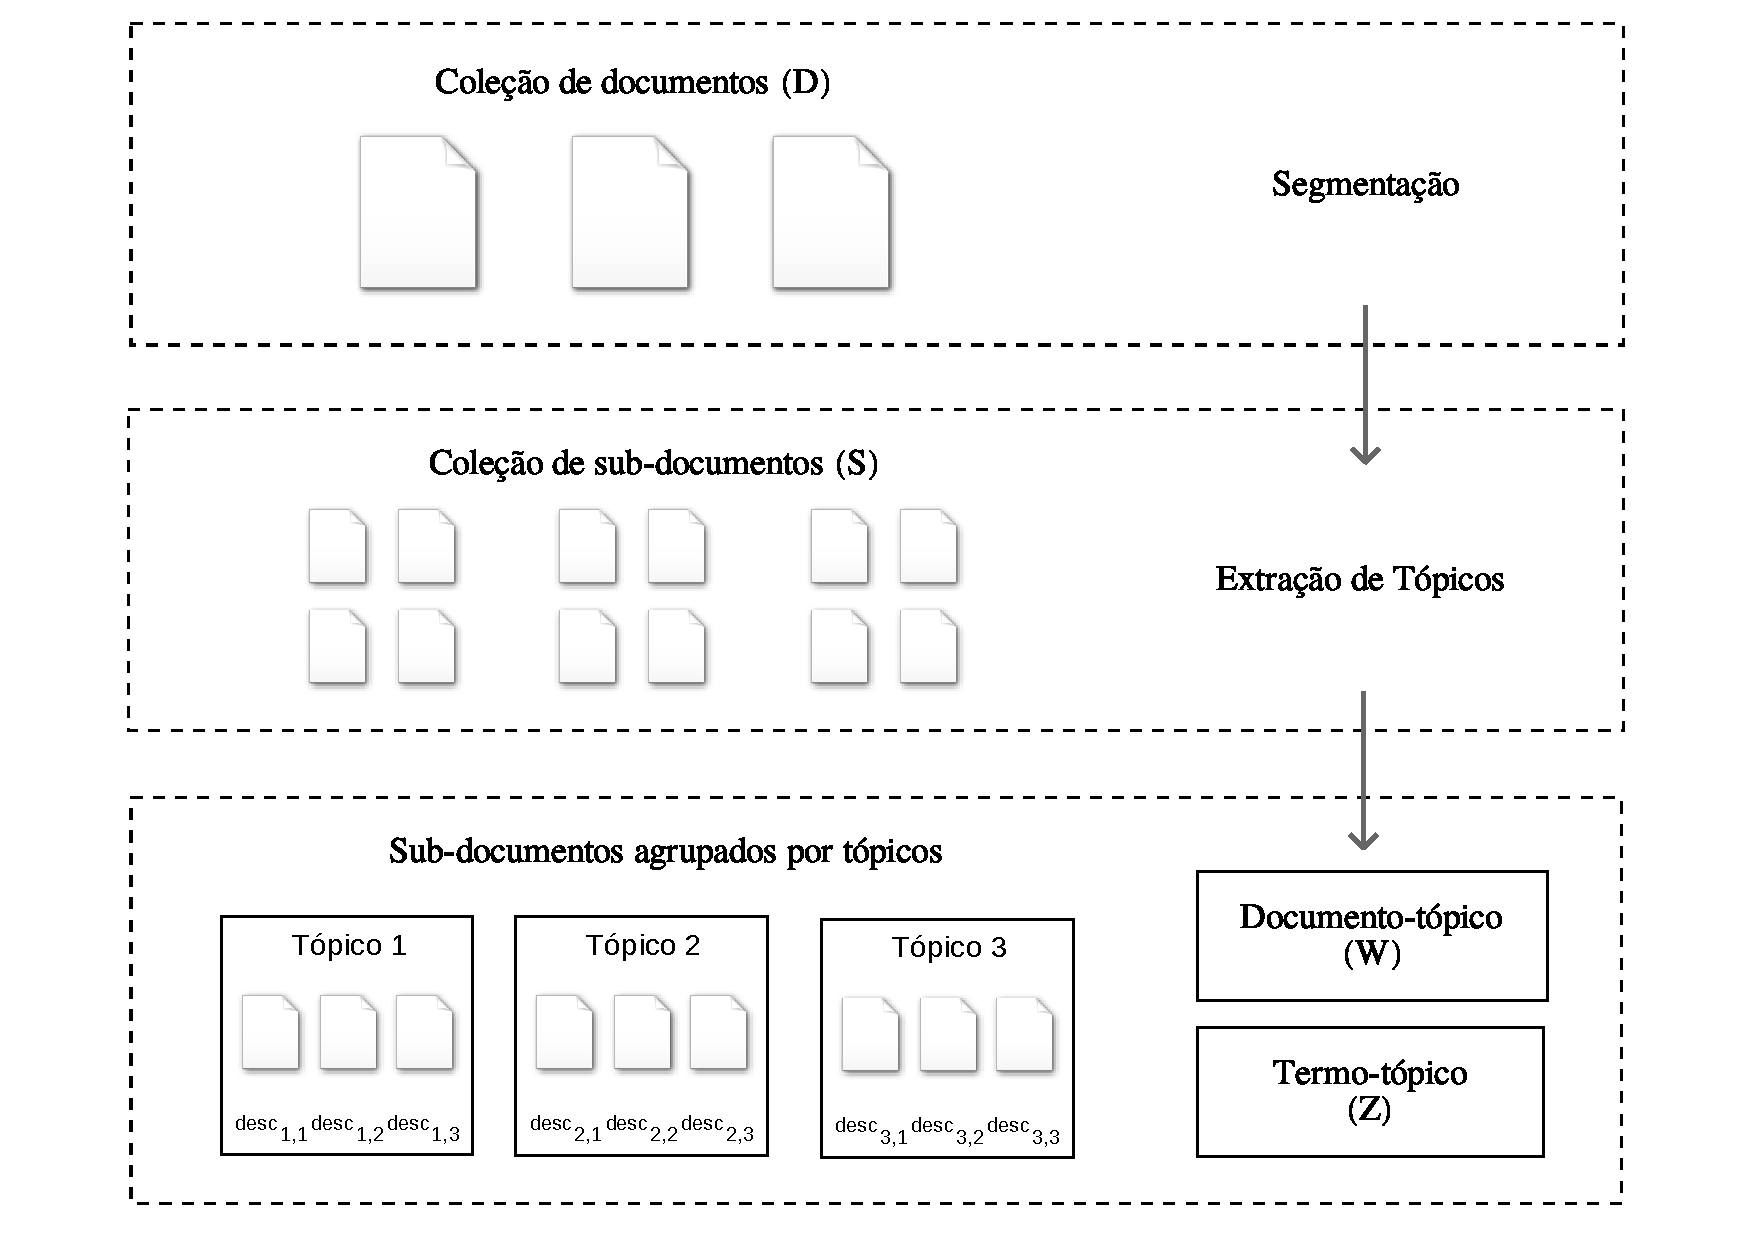
\includegraphics[trim={ 0 40 0 40 },clip,page=1,width=0.9\textwidth]{conteudo/capitulos/figs/estrutura-de-dados-interna.pdf} 

		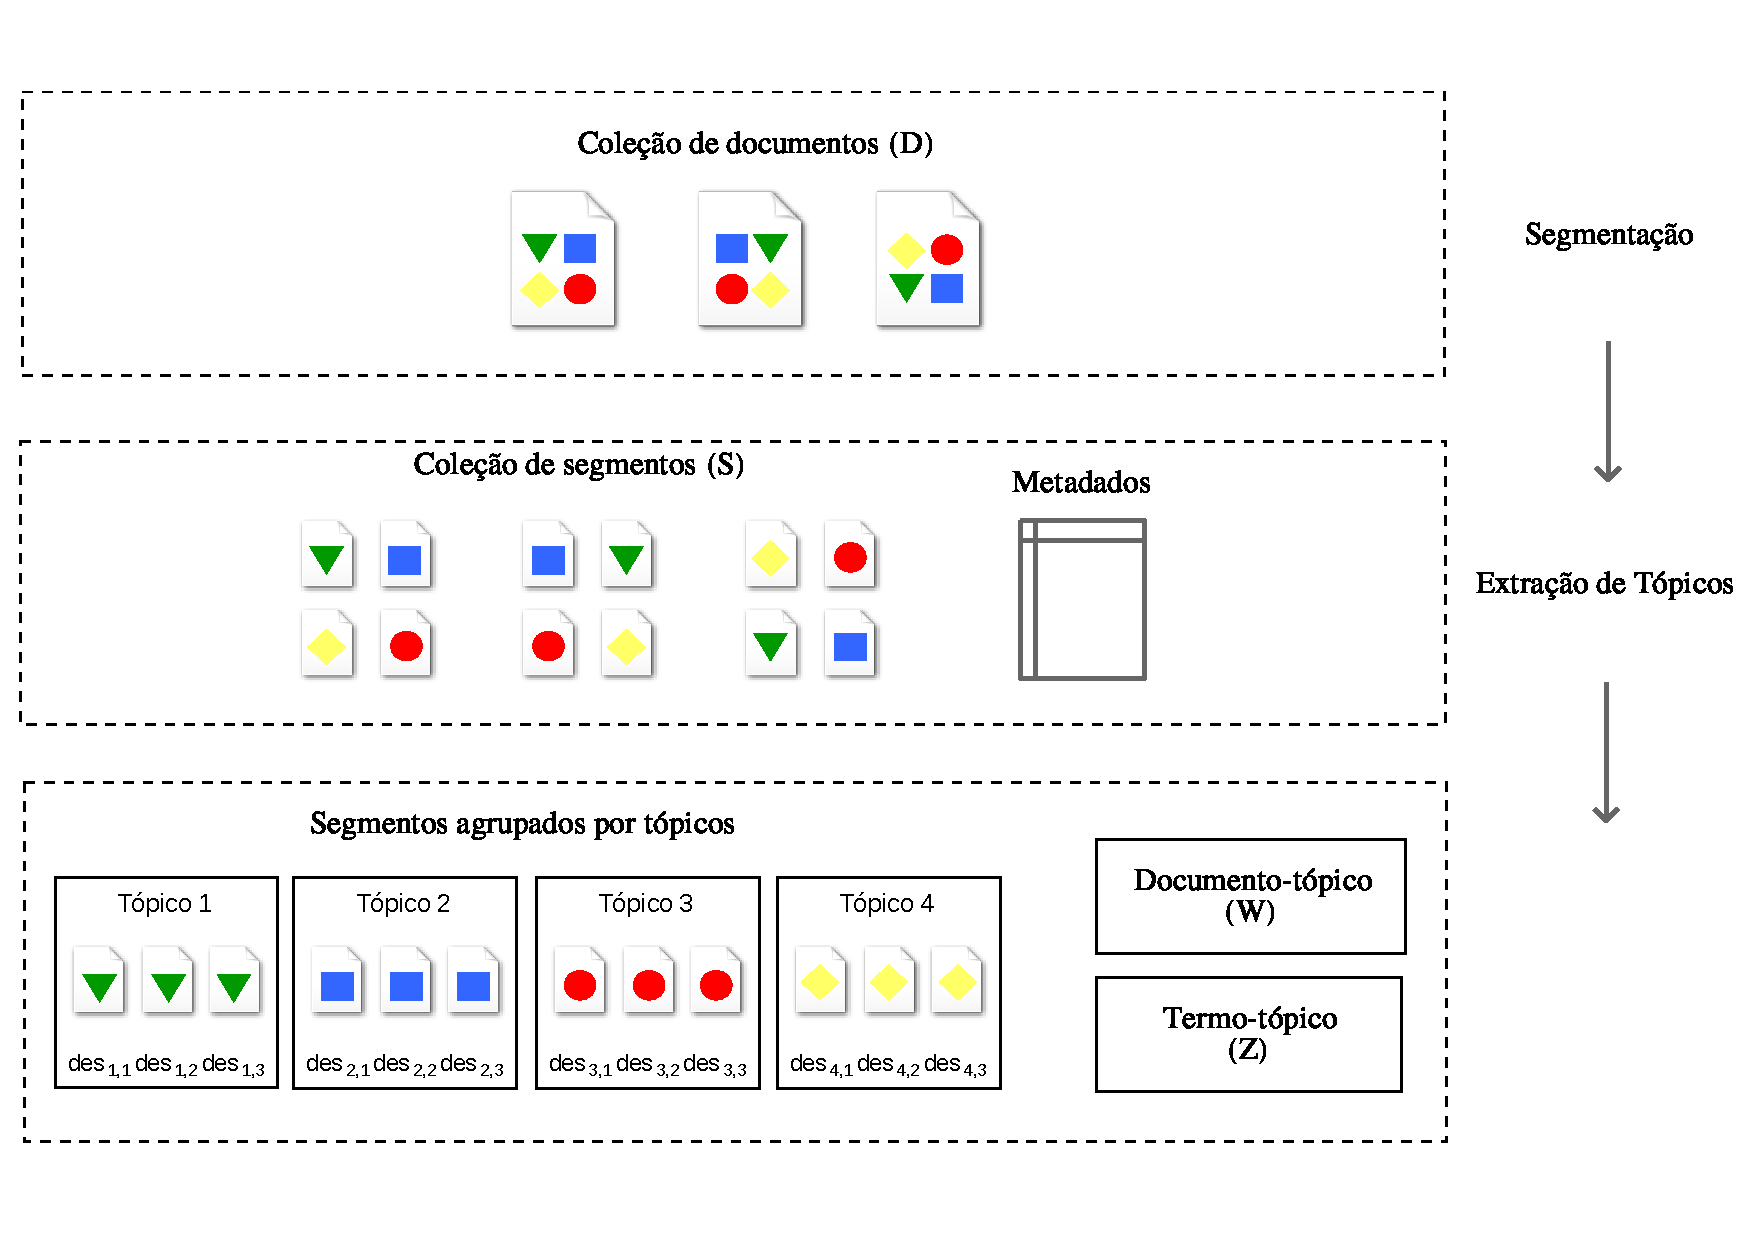
\includegraphics[trim={ 0 40 0 40 },clip,page=1,width=0.9\textwidth]{conteudo/capitulos/figs/estrutura-de-dados-interna-revisada.pdf} 
		\caption{Representação visual da base de dados armazenada pelo sistema e seu processo de geração.}

		% \caption{Visão geral da estrutura de dados interna e seu processo de geração.}
		\label{fig:estrutura-dados-interna}
	\end{figure}




A partir do texto extraído dos documentos originais é gerado o conjunto de segmentos de texto ($S$), armazenados em arquivos de texto plano que contém os textos em formato legível a serem exibidos ao usuário pelo Módulo de Consulta. Para que se conheça o arquivo que deu origem a cada segmento, o sistema gera metadados que mantém a ligação entre os documentos e seus segmentos. 

Os segmentos são então tratados como sub-documentos pelo sistema em que a partir deles o extrator de tópicos irá construir as matrizes documento-tópico ($W$) e termo-tópico ($Z$). Uma vez construídas, essas matrizes são armazenadas em arquivos e usadas para agrupar os segmentos com o mesmo tópico bem como encontrar os melhores termos da coleção para descrever cada tópico.

% Deve-se ressaltar que o sistema recebe um conjunto inicial de documentos a partir do qual a base de dados interna é gerada. A medida que novos documentos são gerados e adicionados ao sistema, serão processados pelo módulo de preparação e manutenção e incorporados a base de dados interna bem como as matrizes documento-tópico e termo-tópicos serão atualizadas pelo extrator de tópicos.




% ==================== Módulo de Consulta ===================== %

\subsection{Módulo de Consulta}


Uma vez que a base de dados interna contém os assuntos abordados na coleção de documentos e o trecho onde se encontram, tem-se um \textit{corpus} derivado do original o qual é melhor organizado e acrescido de informação. A base de dados gerada pelos processos anteriores é então utilizada pelo Módulo de Consulta, cuja responsabilidade é receber a \textit{string} de consulta do usuário, resgatar os dados desejados e apresentá-los em ordem de relevância, dando condições para o usuário acessar os segmentos encontrados, bem como os documentos originais.

\subsubsection{Ranqueamento}
\label{sec-ranqueamento}

Os dados contidos na base de dados interna devem ser acessados por meio de consultas do usuário. Deseja-se que somente os segmentos relevantes sejam exibidos e ordenados por sua similaridade com a consulta. 
Nesse trabalho, a seleção dos segmentos é feita por meio buscas em um espaço vetorial (já apresentado na seção~\ref{subsec:modeloespacovetorial}) onde cada tópico é representado pelos descritores obtidos no processo de extração de tópicos. Essa técnica permite utilizar as variáveis latentes, e fazer com que termos diferentes mas com mesmo significado (polissemia) sejam relacionados e considerados no processo de busca.
Inicialmente, cria-se um \textit{ranking} dos tópicos considerando a similaridade entre seus descritores e a consulta. Em seguida, seleciona-se os tópicos cujos descritores possuem maior relevância com a consulta do usuário e exibe-se os segmentos atribuídos ao primeiro tópico do \textit{ranking}, ficando os demais disponíveis para exploração pelo usuário. 
Os segmentos de cada tópico são ordenados de acordo com o peso atribuído à relação entre o segmento e tópico.  Como resultado, tem-se grupos de segmentos (tópicos) ordenados pela similaridade com a consulta, pelos quais se exibe os segmentos ordenados por sua relevância ao tópico. 
% Essa abordagem é similar aos trabalhos apresentados na Seção~\ref{sec-trabalhos-relacionados}, sendo a principal diferença deste trabalho a técnica de ranqueamento dos resultados.






\subsubsection{Interface}

O sistema deve dar acesso ao usuário para que busque e explore os dados concentrados na base de dados interna, permitindo encontrar resultados relevantes à consulta bem como explorar a base de dados utilizando a organização dos resultados em grupos de segmentos com tópicos relacionados. Deve permitir ao usuário identificar resultados relativante suficientes para compreensão do conteúdo, evitando a leitura de documentos inteiros. Portanto, os textos apresentados devem ser suficientes para compreensão do assunto mencionado, sem necessidade de visualizar o documento original.

A interface desenvolvida para este trabalho foi construída com a finalidade de analisar os resultados de diferentes técnicas de segmentação textual e extração de tópicos. Melhorias nas funcionalidades e usabilidade da interface finais constituem trabalhos futuros relacionados a área de experiência de usuário.

A visualização é divida em 3 painéis principais: (1) campo de busca, onde se insere palavras chave para consulta para um assunto; (2) tópicos encontrados na base de dados; (3) segmentos atribuídos ao tópico selecionado. 
Na Figura~\ref{fig:tela-principal} é apresenta a tela principal do sistema onde observa-se à esquerda os segmentos agrupados por tópicos. Os tópicos são representados por um componente para visualização em árvore e identificados por seus descritores. 
Uma pasta quando expandida revela os segmentos agrupados no tópico que representa. À direita, como resultado da consulta, são apresentados os segmentos selecionados pela relevância com a \textit{string} de busca do usuário. 

  % \begin{figure}[!h]
	  % \centering
	  % 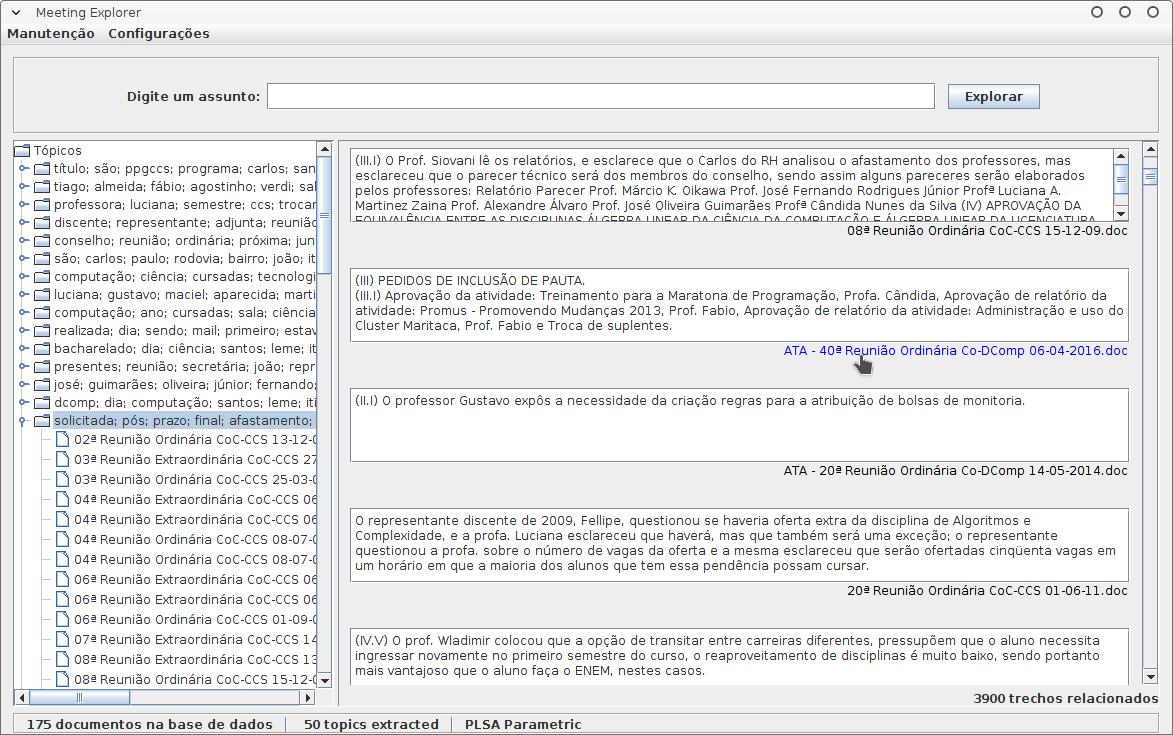
\includegraphics[width=\textwidth]{conteudo/capitulos/figs/tela-principal-2-1.png}
	  % \caption{Tela principal do sistema.}
	  % \label{fig:tela-principal}
  % \end{figure}




O usuário pode reconhecer um tópico por meio dos descritores que ajudam a identificar o assunto pelo qual os segmentos estão relacionados. A qualidade dos descritores e dos grupos extraídos está relacionada ás técnicas de segmentação textual e extração de tópicos empregadas. Nesse sistema, como forma de análise é possível obter resultados de três modelos de extração de tópicos, \textit{K-Means}, \textit{LDA} e \textit{PLSA}, bem como configurá-los manualmente. 
% Na Figura~\ref{fig:configuracaoextratores} é apresentada a interface para configuração do modelo de extração de tópicos. 
Após selecionado um tópico, o sistema apresenta o texto contido em cada segmento a ele atribuído e um \textit{link} para visualizar o arquivo original, como referência. Além disso, ao selecionar um segmento, o sistema destaca outros tópicos aos quais um segmento selecionado está atribuído, permitindo uma forma de exploração à base dados que aproveita o agrupamento de segmentos por assunto.




  \begin{figure}[!h]
	  \centering
	  % 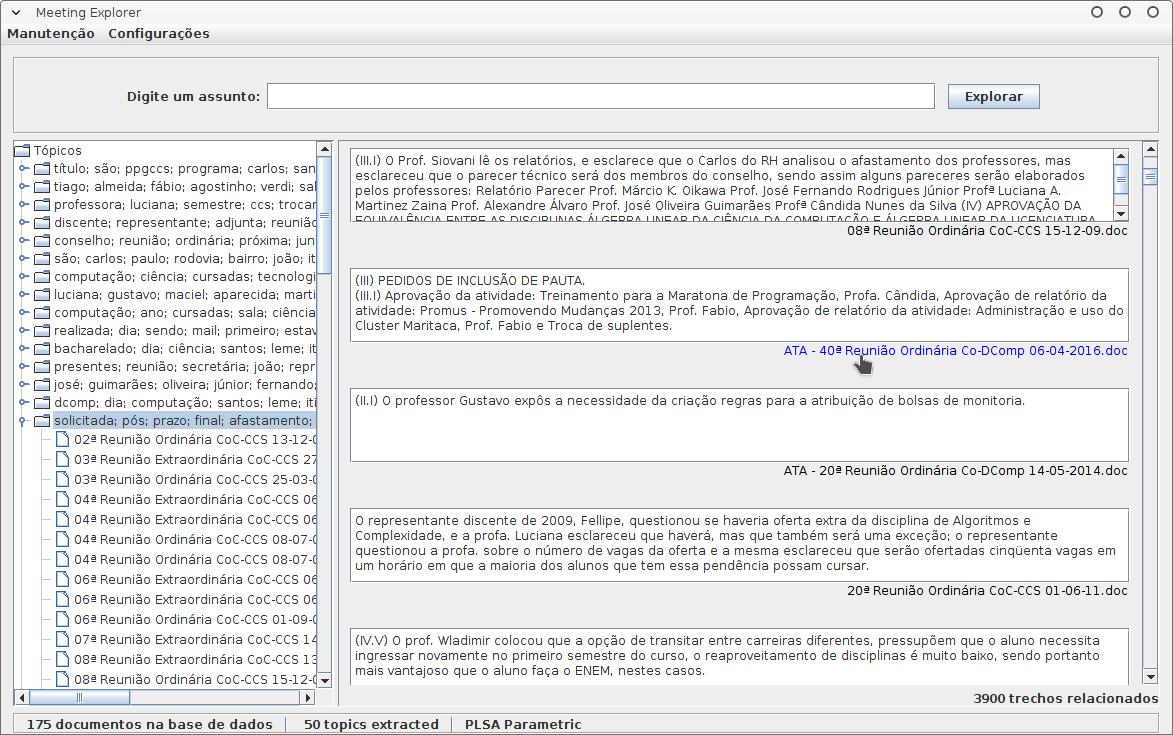
\includegraphics[width=\textwidth]{conteudo/capitulos/figs/tela-principal-2-1.png}
	  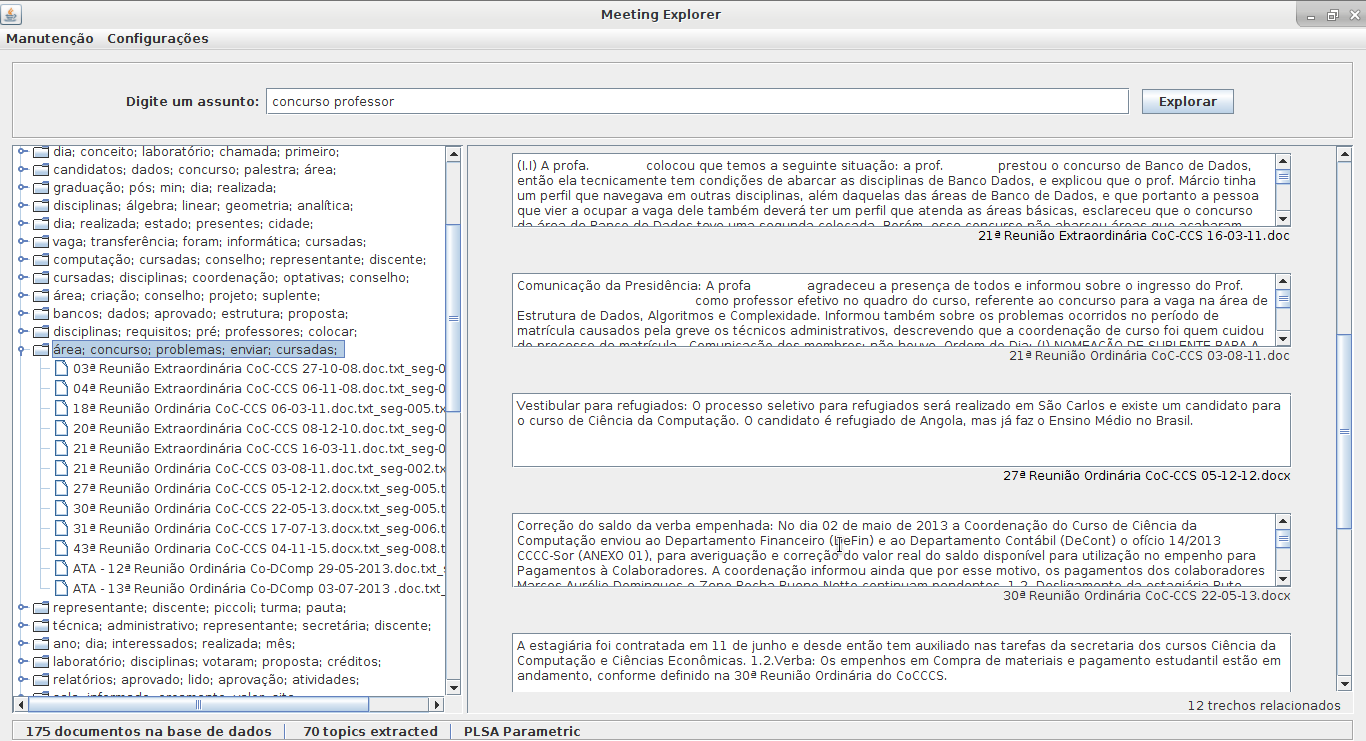
\includegraphics[width=\textwidth]{conteudo/capitulos/figs/consulta.png}
	  % \caption{Tela principal do sistema.}
	  \caption{Tela do sistema que mostra os tópicos e seus respectivos segmentos.}
	  \label{fig:tela-principal}
  \end{figure}


Como parte da proposta, o sistema oferece como opção a ordenação cronológica dos resultados a fim de apresentar cada resultado dentro de um histórico de menções. Dessa forma o usuário tem acesso uma interface que lhe fornece uma visão temporal das menções ao tema pesquisado.
Outras funcionalidades podem ser desejáveis para um sistema voltado a usuários finais, como alternativas à buscas tracionais por palavras-chave, visto que os descritores são uma forma de representação que resume e relaciona o conteúdo dos segmentos, contudo buscas por termos exatos podem ser complementares. 



% As informações apresentadas, incluem dados obtidos do documento como o nome do arquivo, e o texto onde o assunto é mencionado. Além disso, apresenta-se as informação extraídas pelas técnicas de mineração de texto como os descritores e grupos. Para cada busca, é retornada uma lista de resultados ordenados pela relevância com a \textit{string} de entrada, sendo cada item referente a uma menção a um assunto. Um tópico é apresentado em diferentes momentos conforme foi registrado em atas distintas, onde cada menção é um resultado a ser apresentado. 

% Como parte da proposta, o sistema apresenta cada resultado dentro de um histórico de menções. Para isso, abaixo do texto é exibida uma linha com links para os resultados que compartilham o mesmo tópico ordenados por data. Um link, ao ser acionado, direciona para o resultado que aponta, além disso, quando o cursor do mouse está sobre o link, é apresentado um pre-visualização do texto. Dessa forma o usuário tem acesso uma interface que lhe fornece uma visão temporal das menções.

% Uma vez que um item faz menção a um tópico específico, 
% o sistema traz vários resultados para uma consulta, alguns mais relevantes que outros. Para cada resultado (que podem tratar de coisas diferentes) o sistema apresenta um histórico de menções para aquele assunto;




% \section{Estudo de caso}
% \section{Aplicação em um copus de atas de reunião}	
% \section{Validação em um \textit{corpus} de atas de reunião}	
\section{Análise de um \textit{Corpus} de Atas de Reunião Utilizando Ferramentas do Sistema}	
\label{sec:aplicacao-sistema}

O foco principal deste projeto de mestrado é a exploração e recuperação de informação em atas de reunião. 
% A escolha foi feita baseada nas 
% 
As atas de reunião, em geral, apresentam como característica textos relativamente curtos, em comparação com outros documentos como notícias, artigos, sites da \textit{web}; o estilo de escrita formal em que o redator evita repetições de temos e conceitos em benefício da estética do texto; Multiplicidade de assuntos contidos em uma mesma ata, na qual é difícil determinar um assunto central, mas diversos assuntos independentes que foram tratados durante a reunião.
A literatura pesquisada apresenta poucos trabalhos voltados à essas caraterísticas, sobre tudo para o idioma português. Assim, escolheu-se um \textit{corpus} de atas de reunião com propósito principal de contribuir com ferramentas e conhecimentos nesse sentido. 
% esse trabalho tem foco em atas de 
% reunião c

% características desses documentos como 


A seguir, será descrito o conjunto de atas de reunião utilizado como base de dados e os resultados obtidos pela aplicação das técnicas são observados para compreensão e análise do \textit{corpus} estudado.




\subsection{Composição do \textit{Corpus} }
\label{subsec:composicaocorpus}

O \textit{corpus} abordado nesse trabalho foi formado por atas de reunião coletadas da Universidade Federal de São Carlos - Campus Sorocaba. 
Coletou-se 175 atas públicas
% da Universidade Federal de São Carlos - Campus Sorocaba, destas, são 
das quais são 
66 do Conselho do Departamento de Computação, sendo 55 referentes a reuniões ordinárias e 11 extraordinárias;
73 do Conselho do Curso de Bacharelado em Ciência da Computação, sendo 42 referentes a reuniões ordinárias e 31 extraordinárias e
36 da Comissão do Curso de Pós-Graduação em Ciência da Computação, sendo 31 referentes a reuniões ordinárias e 5 extraordinárias.
As referentes a reuniões ordinárias têm em média 827 \textit{tokens} enquanto as extraordinárias têm 667 \textit{tokens} em média.

As atas de reunião diferem dos textos comumente estudados em outros trabalhos em alguns pontos. Frequentemente atas de reunião têm a característica de apresentar um texto com poucas quebras de parágrafo e sem marcações de estrutura, como capítulos, seções ou quaisquer indicações sobre o tema do texto. Além disso, possuem estilo de escrita bastante sucinto, em que o redator evita repetições de palavras em favor da estética do texto. O estilo de escrita formal mais compacto, pode dificultar processos de mineração de texto~\cite{Choi2001-LSA}.  % alguns processos








\subsection{Exploração e Observação do \textit{Corpus}}

Como retorno, diferentes modelos de extração de tópicos apresentam resultados distintos em relação aos descritores e segmentos atribuídos a cada tópico. Na Tabela~\ref{tab:resumodescritoreseqtdsegmetnos} é apresentado um resumo dos tópicos extraídos do \textit{corpus} por cada modelo. Os dados foram gerados configurando cada modelo para extrair um total de 70 tópicos da base da coleção, onde se observa 3 descritores extraídos para cada tópico. Os tópicos estão ordenados pela quantidade de segmentos atribuídos dos quais são exibidos os 45 primeiros tópicos. Os resultados completos dessa tabela, com 70 tópicos e 5 descritores podem ser vistos no Apêndice~\ref{apendice3}.



% \begin{table}[!h]
% \center
	% 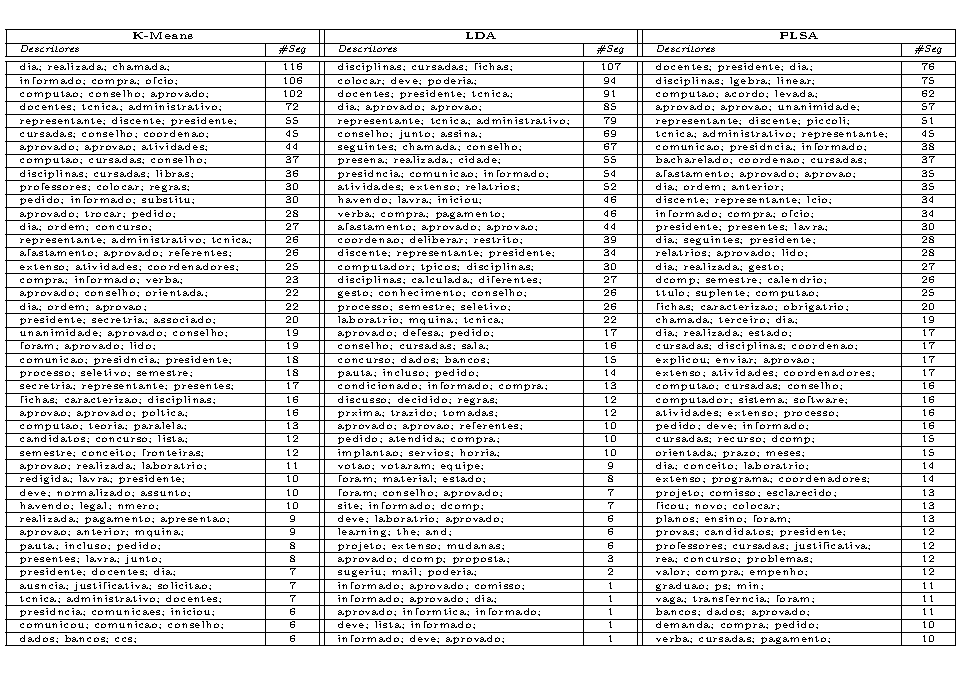
\includegraphics[page=1,width=1\textwidth]{anexos/tabelas/distribuicao-topicos/distribuicao-topicos-resumo.pdf}
 % \caption{Descritores e número de segmentos no tópico selecionado pelos Algoritmos}
 % \label{tab:resumodescritoreseqtdsegmetnos}
% \end{table} 

\begin{landscape}% Landscape page
% \tiny

\begin{table}[!h]
\tiny
	\centering
	\begin{tabular}{|l|c||l|c||l|c|} \hline

		\multicolumn{2}{|c||}{ \textbf{K-Means} } & \multicolumn{2}{c||}{ \textbf{LDA} } & \multicolumn{2}{c|}{ \textbf{PLSA} } \\ \hline
		\textit{Descritores} & \textit{\#Seg} & \textit{Descritores} & \textit{\#Seg} & \textit{Descritores} & \textit{\#Seg} \\ \hline
\hline
   dia; realizada; chamada; &   116  &         disciplinas; cursadas; fichas; &   107  &       docentes; presidente; dia; &   76   \\ \hline
   informado; compra; ofício; &   106  &         colocar; deve; poderia; &   94  &       disciplinas; álgebra; linear; &   75  \\ \hline
   computação; conselho; aprovado; &   102  &         docentes; presidente; técnica; &   91  &       computação; acordo; levada; &   62  \\ \hline
   docentes; técnica; administrativo; &   72  &         dia; aprovado; aprovação; &   85  &       aprovado; aprovação; unanimidade; &   57  \\ \hline
   representante; discente; presidente; &   55  &         representante; técnica; administrativo; &   79  &       representante; discente; piccoli; &   51  \\ \hline
   cursadas; conselho; coordenação; &   45  &         conselho; junto; assina; &   69  &       técnica; administrativo; representante; &   45  \\ \hline
   aprovado; aprovação; atividades; &   44  &         seguintes; chamada; conselho; &   67  &       comunicação; presidência; informado; &   38  \\ \hline
   computação; cursadas; conselho; &   37  &         presença; realizada; cidade; &   55  &       bacharelado; coordenação; cursadas; &   37  \\ \hline
   disciplinas; cursadas; libras; &   36  &         presidência; comunicação; informado; &   54  &       afastamento; aprovado; aprovação; &   35  \\ \hline
   professores; colocar; regras; &   30  &         atividades; extensão; relatórios; &   52  &       dia; ordem; anterior; &   35  \\ \hline
   pedido; informado; substituí; &   30  &         havendo; lavra; iniciou; &   46  &       discente; representante; lúcio; &   34  \\ \hline
   aprovado; trocar; pedido; &   28  &         verba; compra; pagamento; &   46  &       informado; compra; ofício; &   34  \\ \hline
   dia; ordem; concurso; &   27  &         afastamento; aprovado; aprovação; &   44  &       presidente; presentes; lavra; &   30  \\ \hline
   representante; administrativo; técnica; &   26  &         coordenação; deliberar; restrito; &   39  &       dia; seguintes; presidente; &   28  \\ \hline
   afastamento; aprovado; referentes; &   26  &         discente; representante; presidente; &   34  &       relatórios; aprovado; lido; &   28  \\ \hline
   extensão; atividades; coordenadores; &   25  &         computador; tópicos; disciplinas; &   30  &       dia; realizada; gestão; &   27  \\ \hline
   compra; informado; verba; &   23  &         disciplinas; calculada; diferentes; &   27  &       dcomp; semestre; calendário; &   26  \\ \hline
   aprovado; conselho; orientada; &   22  &         gestão; conhecimento; conselho; &   26  &       título; suplente; computação; &   25  \\ \hline
   dia; ordem; aprovação; &   22  &         processo; semestre; seletivo; &   26  &       fichas; caracterização; obrigatório; &   20  \\ \hline
   presidente; secretária; associado; &   20  &         laboratório; máquina; técnica; &   22  &       chamada; terceiro; dia; &   19  \\ \hline
   unanimidade; aprovado; conselho; &   19  &         aprovado; defesa; pedido; &   17  &       dia; realizada; estado; &   17  \\ \hline
   foram; aprovado; lido; &   19  &         conselho; cursadas; sala; &   16  &       cursadas; disciplinas; coordenação; &   17  \\ \hline
   comunicação; presidência; presidente; &   18  &         concurso; dados; bancos; &   15  &       explicou; enviar; aprovação; &   17  \\ \hline
   processo; seletivo; semestre; &   18  &         pauta; inclusão; pedido; &   14  &       extensão; atividades; coordenadores; &   17  \\ \hline
   secretária; representante; presentes; &   17  &         condicionado; informado; compra; &   13  &       computação; cursadas; conselho; &   16  \\ \hline
   fichas; caracterização; disciplinas; &   16  &         discussão; decidido; regras; &   12  &       computador; sistema; software; &   16  \\ \hline
   aprovação; aprovado; política; &   16  &         próxima; trazido; tomadas; &   12  &       atividades; extensão; processo; &   16  \\ \hline
   computação; teoria; paralela; &   13  &         aprovado; aprovação; referentes; &   10  &       pedido; deve; informado; &   16  \\ \hline
   candidatos; concurso; lista; &   12  &         pedido; atendida; compra; &   10  &       cursadas; recurso; dcomp; &   15  \\ \hline
   semestre; conceito; fronteiras; &   12  &         implantação; serviços; horária; &   10  &       orientada; prazo; meses; &   15  \\ \hline
   aprovação; realizada; laboratório; &   11  &         votação; votaram; equipe; &   9  &       dia; conceito; laboratório; &   14  \\ \hline
   redigida; lavra; presidente; &   10  &         foram; material; estado; &   8  &       extensão; programa; coordenadores; &   14  \\ \hline
   deve; normalizado; assunto; &   10  &         foram; conselho; aprovado; &   7  &       projeto; comissão; esclarecido; &   13  \\ \hline
   havendo; legal; número; &   10  &         site; informado; dcomp; &   7  &       ficou; novo; colocar; &   13  \\ \hline
   realizada; pagamento; apresentação; &   9  &         deve; laboratório; aprovado; &   6  &       planos; ensino; foram; &   13  \\ \hline
   aprovação; anterior; máquina; &   9  &         learning; the; and; &   6  &       provas; candidatos; presidente; &   12  \\ \hline
   pauta; inclusão; pedido; &   8  &         projeto; extensão; mudanças; &   6  &       professores; cursadas; justificativa; &   12  \\ \hline
   presentes; lavra; junto; &   8  &         aprovado; dcomp; proposta; &   3  &       área; concurso; problemas; &   12  \\ \hline
   presidente; docentes; dia; &   7  &         sugeriu; mail; poderia; &   2  &       valor; compra; empenho; &   12  \\ \hline
   ausência; justificativa; solicitação; &   7  &         informado; aprovado; comissão; &   1  &       graduação; pós; min; &   11  \\ \hline
   técnica; administrativo; docentes; &   7  &         informado; aprovado; dia; &   1  &       vaga; transferência; foram; &   11  \\ \hline
   presidência; comunicações; iniciou; &   6  &         aprovado; informática; informado; &   1  &       bancos; dados; aprovado; &   11  \\ \hline
   comunicou; comunicação; conselho; &   6  &         deve; lista; informado; &   1  &       demanda; compra; pedido; &   10  \\ \hline
   dados; bancos; ccs; &   6  &         informado; deve; aprovado; &   1  &       verba; cursadas; pagamento; &   10  \\ \hline
   informática; sociedade; docentes; &   6  &         deve; informática; conselho; &   1  &       laboratório; manutenção; suplente; &   10  \\ \hline
   % estudos; liberados; instalação; &   6  &         conselho; informado; dia; &   1  &       área; criação; conselho; &   9  \\ \hline
   % processo; participação; ficou; &   6  &         conselho; dia; aprovado; &   1  &       laboratório; disciplinas; votaram; &   9  \\ \hline
   % extensão; atividades; coordenadores; &   6  &         informática; conselho; informado; &   1  &       disciplinas; cursadas; oferta; &   9  \\ \hline
   % presidência; informado; comunicação; &   5  &         aprovado; deve; informado; &   1  &       manutenção; informado; laboratório; &   9  \\ \hline
   % votaram; conselho; favor; &   5  &         informática; informado; conselho; &   1  &       colocar; lecionar; disciplinas; &   9  \\ \hline
   % iniciou; poderia; gestante; &   5  &         conselho; informado; aprovado; &   1  &       laboratório; conselho; colocar; &   9  \\ \hline
   % unidades; positivo; leitura; &   5  &         aprovado; conselho; informado; &   1  &       estágio; cursadas; atividades; &   8  \\ \hline
   % discussão; dcomp; normalizado; &   5  &         deve; dia; bolsa; &   1  &       colocar; diz; esclarecido; &   8  \\ \hline
   % havendo; trata; deus; &   5  &         informado; conselho; deve; &   1  &       conselho; computação; cursadas; &   7  \\ \hline
   % votação; entrou; solicitada; &   5  &         aprovado; unanimidade; conselho; &   1  &       candidatos; dados; concurso; &   6  \\ \hline
   % recurso; foram; adequação; &   5  &         próxima; informado; aprovado; &   1  &       sala; informado; orçamento; &   6  \\ \hline
   % avaliação; extensão; discussão; &   5  &         aprovado; deve; dcomp; &   1  &       proposta; colocar; copq; &   6  \\ \hline
   % associado; presidente; chistine; &   4  &         conselho; informado; dia; &   1  &       cursadas; existam; pedido; &   6  \\ \hline
   % persianas; pedido; foram; &   4  &         palestra; apoio; sustentabilidade; &   1  &       bolsa; cursadas; distribuição; &   6  \\ \hline
   % estágio; apresentação; secretário; &   4  &         próxima; conselho; discussão; &   1  &       disciplinas; tem; colocar; &   6  \\ \hline
   % gestão; ambiental; noções; &   4  &         informado; conselho; dia; &   1  &       presidente; discussão; cursadas; &   5  \\ \hline
   % piccoli; ausência; justificativa; &   4  &         implantação; horária; serviços; &   1  &       junto; assina; participante; &   5  \\ \hline
   % calendário; apresentar; dcomp; &   4  &         informado; deve; transferência; &   1  &       colocar; verba; poderia; &   5  \\ \hline
   % sistema; técnica; relatórios; &   3  &         aprovado; dia; conselho; &   1  &       chefia; seriam; criar; &   5  \\ \hline
   % gasto; verba; custeio; &   3  &         participação; evento; palestra; &   1  &       capacitação; afastamento; regras; &   5  \\ \hline
   % sistema; operacionais; ccs; &   3  &         comissão; eleição; aprovado; &   1  &       seriam; edital; colocar; &   5  \\ \hline
   % semana; estudos; perfil; &   2  &         deve; dia; conselho; &   1  &       cursadas; proposta; atividades; &   4  \\ \hline
   % professores; férias; resposta; &   2  &         conselho; informado; substituição; &   1  &       ano; dia; interessados; &   3  \\ \hline
   % moraes; assunto; trata; &   2  &         dia; deve; conselho; &   1  &       projeto; foram; pesos; &   3  \\ \hline
   % fapesp; rti; cocccs; &   2  &         conselho; pedido; dia; &   1  &       disciplinas; requisitos; pré; &   1  \\ \hline

	\end{tabular}
	% \caption{Resumo dos tópicos obtidos com os extratores \textit{K-Means}, \textit{LDA} e \textit{PLSA}. 
% As linhas representam os tópicos, para os quais são mostrados 5 descritores e a quantidade de segmentos atribuídos.
	% Para cada extrator é mostrado 5 descritores e a quantidade de documentos atribuídos a cada tópico.
% }
	% \label{tab:resumo-resultados}
 \caption{Descritores e número de segmentos no tópico selecionado pelos Algoritmos}
 \label{tab:resumodescritoreseqtdsegmetnos}
\end{table}




\end{landscape}




De maneira geral, os retornos do sistema apresentados na Tabela~\ref{tab:resumodescritoreseqtdsegmetnos} oferecem uma perspectiva, segundo os modelos utilizados, dos principais assuntos abordados no \textit{corpus}. Por exemplo, o termo \textit{``aprovado''} e \textit{``aprovação''} aparecem como descritores de vários dos tópicos mais numerosos, o que indica que grande parte dos segmentos, abordam assuntos relacionados a aprovações pelos membros da reunião. De forma semelhante, as frequências de termos como \textit{``compra''} e \textit{``verba''}, podem mostrar a importância desses termos para o ambiente onde se deram as reuniões.


Observou-se também que alguns tópicos concentram segmentos considerados pouco relevantes em termos de conteúdo, como a primeira parte introdutória da ata, onde se registra informações como data, local, membros e departamento. Esses segmentos são identificados com os termos 
\textit{``dia; realizada; chamada;''} pelo K-Means com 116 segmentos; 
\textit{``seguintes; chamada; conselho;''} pelo LDA com 67 segmentos e 
\textit{``dia; realizada; gestão;''} e \textit{``dia; seguintes; presidente;''} pelo PLSA com 28 e 27 segmentos. Vale salientar que os segmentos possuem texto similar, porém não idênticos e que os cabeçalhos e rodapés não estão presentes uma vez que foram removidos na etapa de preparação dos documentos. Como parte da proposta desse trabalho, esse agrupamento ajuda identificar textos com pouca relevância em termos de assuntos abordados na reunião.
Os resultados dos sistema são melhores analisados no capítulos~\ref{cap-segmentadores}~e~\ref{cap-extratores} onde as técnicas de segmentação textual e extração de tópicos são avaliadas no contexto das atas de reunião.


Os dados obtidos pela aplicação das técnicas permitem analisar o \textit{corpus} pela distribuição dos tópicos ao longo da coleção de documentos identificando os assuntos em cada segmento de ata individualmente, gerando assim uma perspectiva ampla dos assuntos contidos na coleção de documentos. Além disso, essa metodologia pode dar uma visão da distribuição dos tópicos em cada um dos documentos. Na Figura~\ref{fig:distribuicao-ata} é exibido graficamente a distribuição de 6 tópicos extraídos de uma ata da coleção. 


  % \begin{center}
	% \begin{figure}[h!]

		% 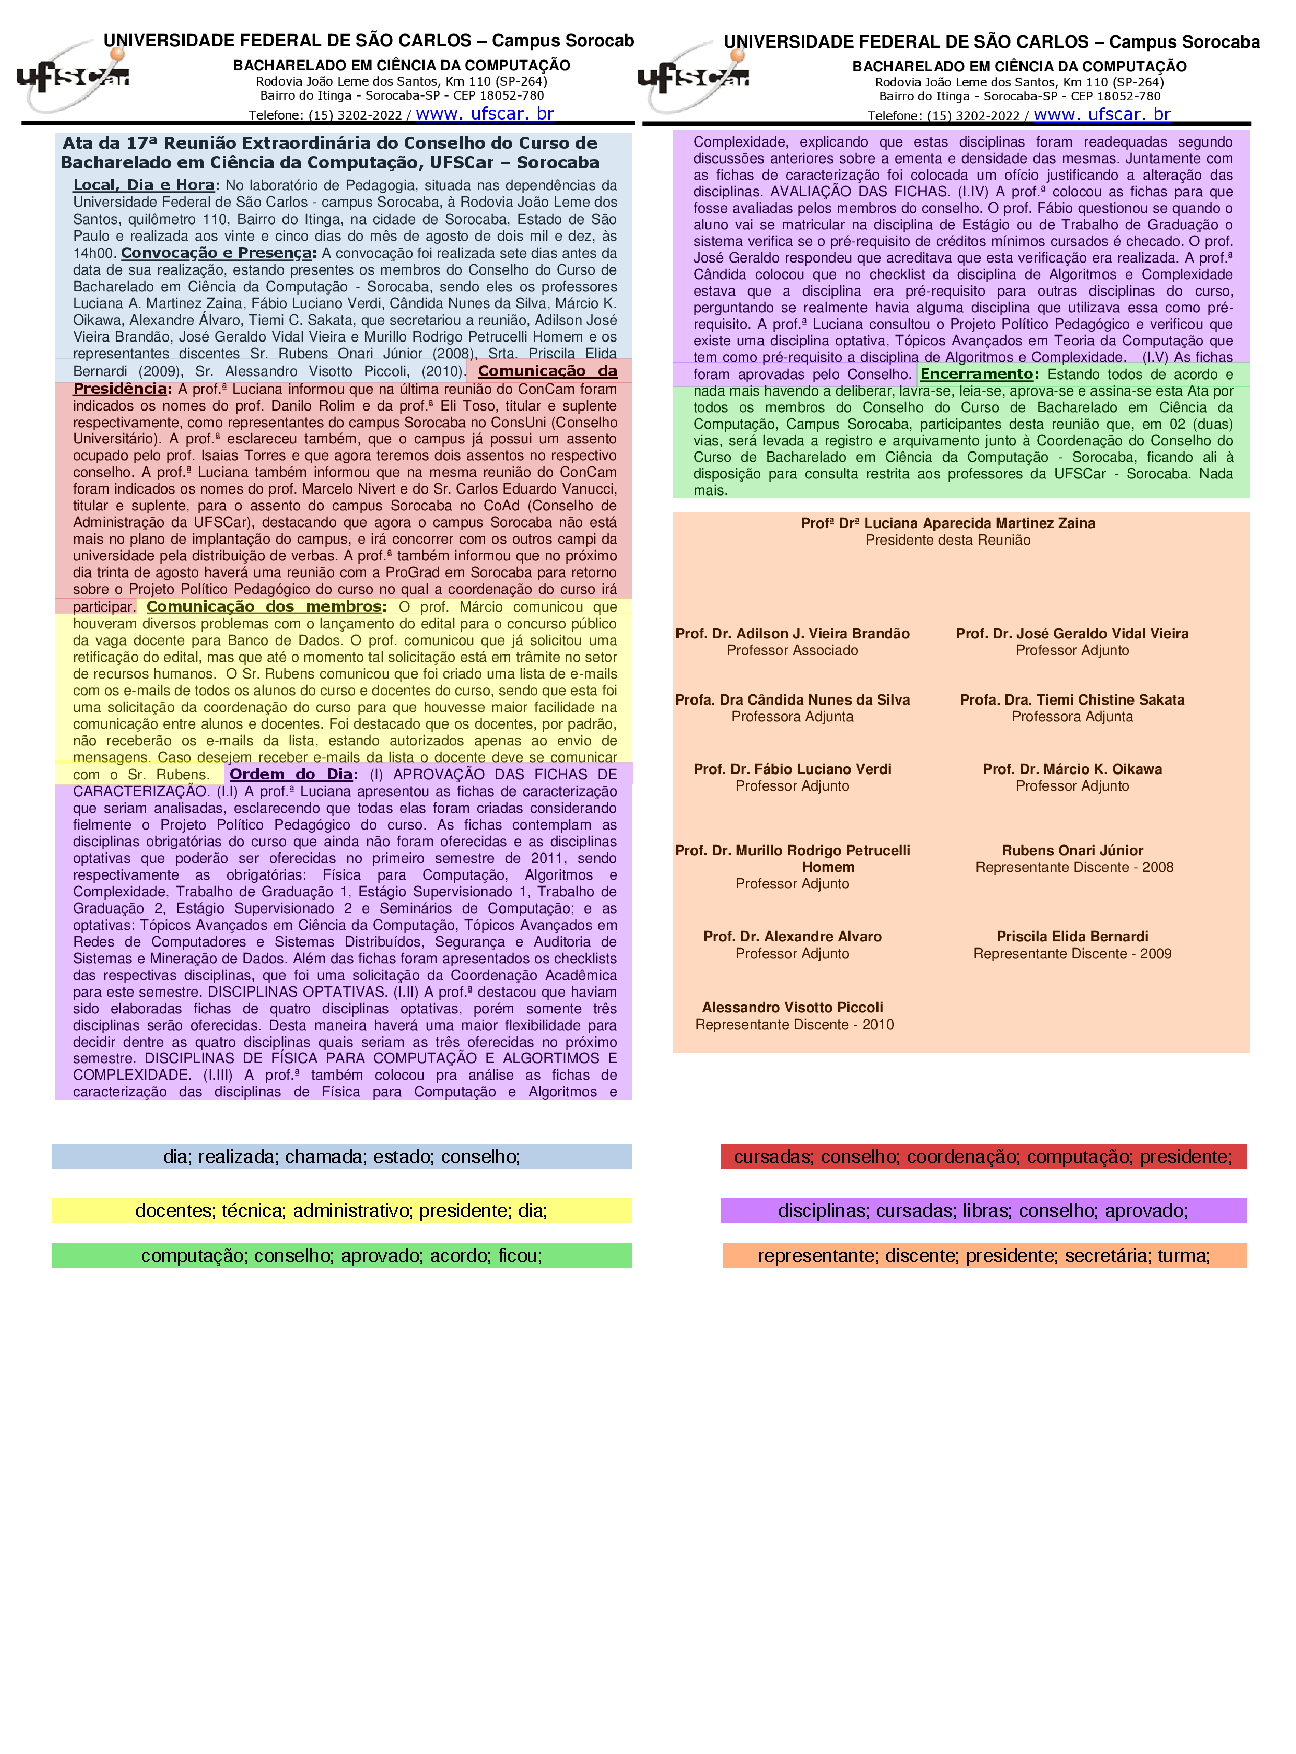
\includegraphics[trim={ 0 235 0 0 },clip,page=1,width=\textwidth]{conteudo/capitulos/figs/doc-em-png/distribuicao.pdf}

		% \caption{Distribuição de tópicos em uma ata real. Cada tópico é representado por uma região colorida. Abaixo estão os descritores identificados pela cor do respectivo tópico. Os nomes de pessoas foram ocultados por não expressarem significado nesse trabalho.}
		% \label{fig:distribuicao-ata}
	% \end{figure}
% \end{center}


A ata exibida, foi segmentada utilizando algoritmo \textit{BayesSeg} e os tópicos da coleção foram extraídos com o \textit{K-Means}. Como já mencionado, as primeiras sentenças referem-se a introdução e apresentação da própria reunião e seus membros, as quais o extrator atribuiu a um grupo com 116 segmentos com os descritores \textit{``dia; realizada; chamada; estado; conselho;''}. De forma semelhante, a região da ata reservada à assinatura dos membros foi atribuída a um grupo com 55 segmentos identificados pelos termos \textit{``representante; discente; presidente; secretária; turma;''}. 



  \begin{center}
	\begin{figure}[h!]

		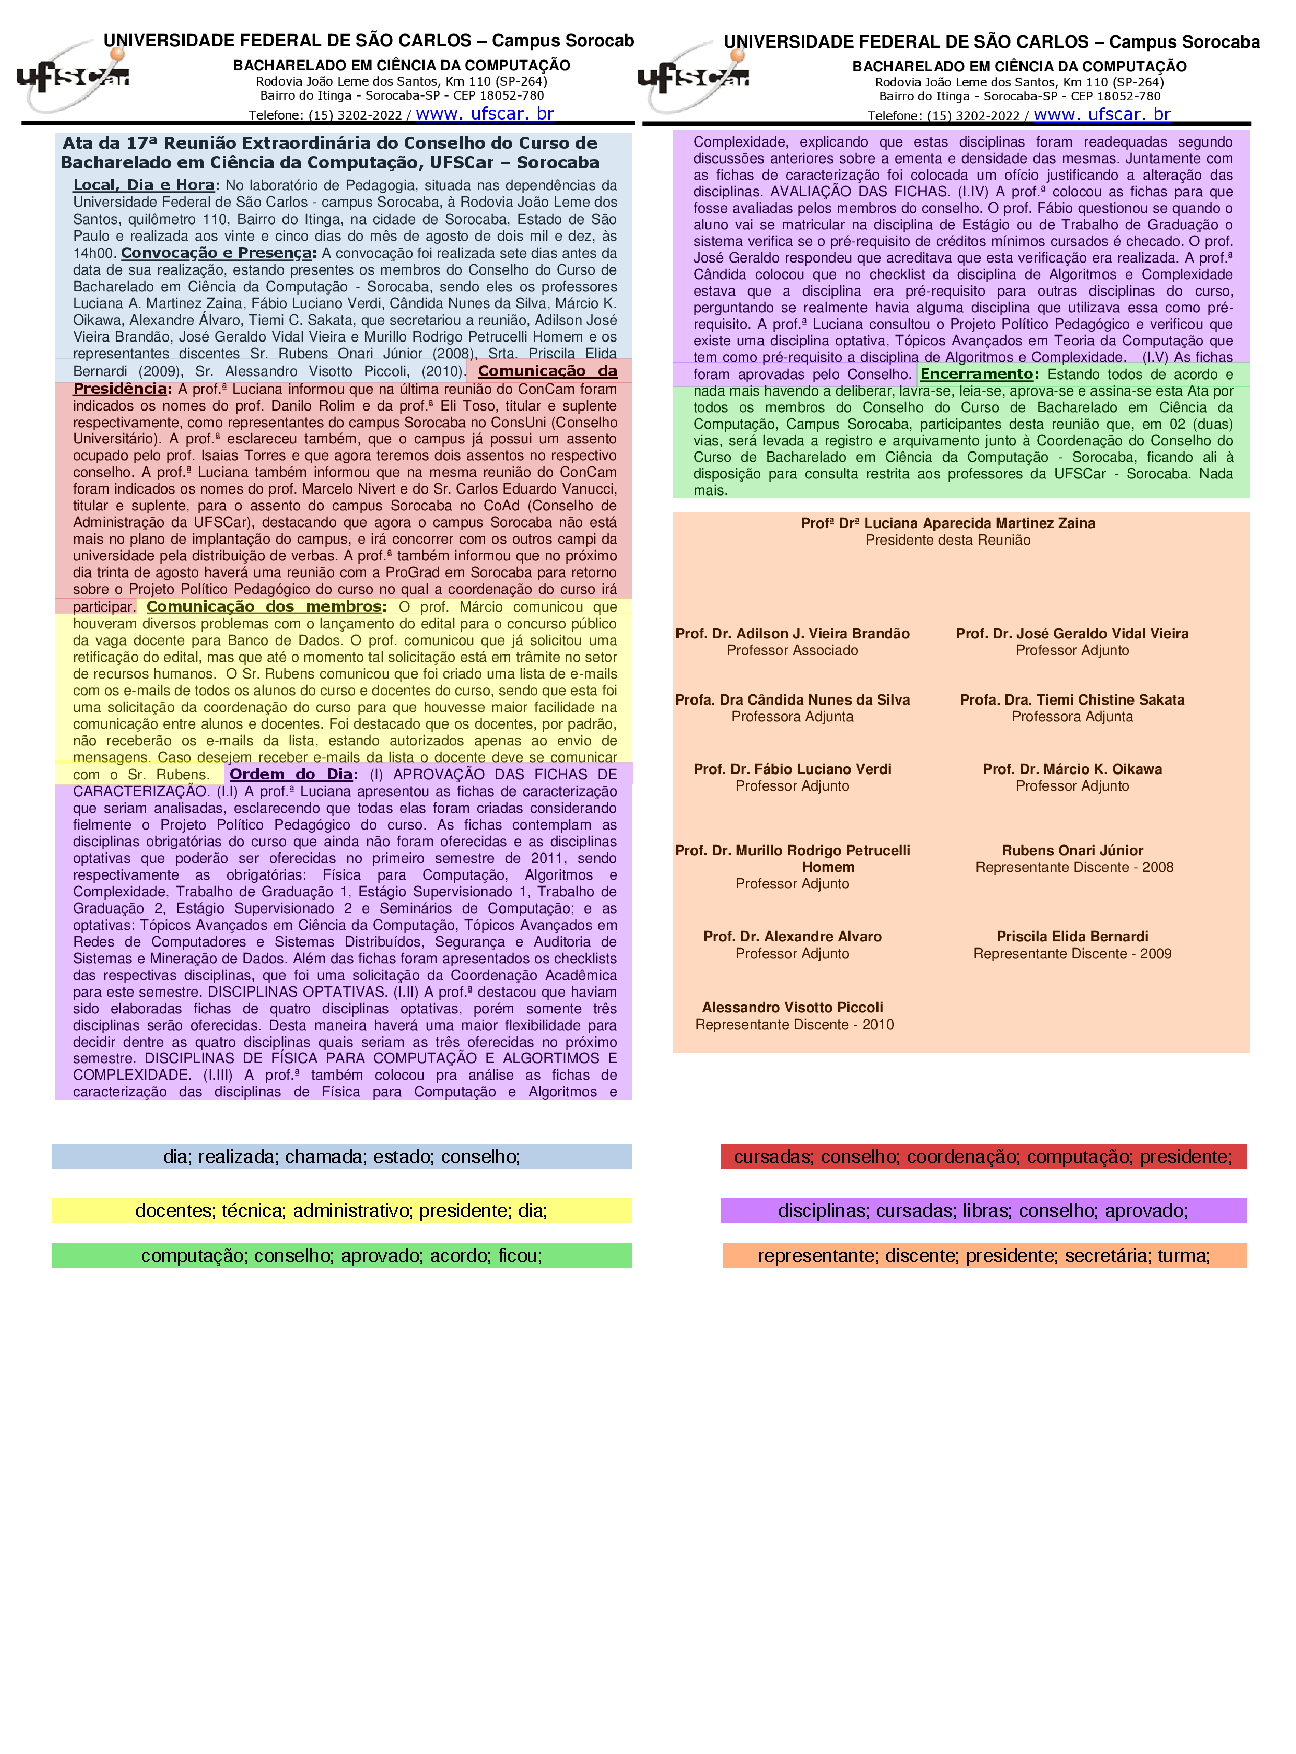
\includegraphics[trim={ 0 235 0 0 },clip,page=1,width=\textwidth]{conteudo/capitulos/figs/doc-em-png/distribuicao.pdf}

		\caption{Distribuição de tópicos em uma ata real. Cada tópico é representado por uma região colorida. Abaixo estão os descritores identificados pela cor do respectivo tópico. Os nomes de pessoas foram ocultados por não expressarem significado nesse trabalho.}
		\label{fig:distribuicao-ata}
	\end{figure}
\end{center}




\section{Considerações Finais}

Nessa seção foi apresentado o sistema desenvolvido desde sua proposta original, as principais técnicas que o compõe, bem como sua aplicação em um \textit{corpus} formado por atas de reunião. O sistema apresentado tem como escopo inicial a análise das técnicas de segmentação textual e modelos de extração de tópicos com documentos formados por múltiplos assuntos sem meta informações. 

O sistema mostrou-se capaz de criar e manter uma base de dados estruturada a partir de documentos textuais não estruturados e utilizá-la para incorporar e  recuperar informações úteis. Usando técnicas de Recuperação de Informação foi possível localizar grupos e segmentos relevantes às consultas bem como estabelecer rankings com resultados mais pertinentes.

Os agrupamentos e descritores  atribuídos aos segmentos permitem ao usuário visualizar os principais assuntos contidos na coleção de documentos, além de perceber relações latentes entre esses assuntos. As estrutura criada fornece uma representação que pode descrever o conteúdo dos segmentos das atas para exploração do usuário, bem como para técnicas de Recuperação de Informação. Mais análises voltadas aos resultados do sistema são discutidas no Capítulo~\ref{cap-segmentadores} e no Capítulo~\ref{cap-extratores}. Trabalhos futuros relacionados ao sistema e à metodologia empregada são abordados no Capítulo~\ref{cap:conclusao}.

% -- qual o ganho em relação a um sitema de busca por palavras-chave? 





























